
\chapter{Introduction}\label{chap:introduction}

The purpose of this work is to investigate the use of a novel quantized state method for the time-domain simulation of electrical power systems, and to determine if this method is a feasible and advantageous approach to simulating power system dynamics compared to the current state-of-the-art methods. 

\section{The Proposed Simulation Method: QDL}

The proposed modeling and simulation method combines three concepts: the Latency Insertion Method (LIM), Quantized Discrete Event Specification (QDEVS), and Quantized State Systems (QSS). The method is therefore called QDEVS-LIM, (abbreviated throughout this document as QDL). The LIM, described in \cite{schutt2001}, can be thought of as a system partitioning method, such as using Bergeron transmission lines to decouple large electrical network models by exploiting the latency inherent to long transmission lines. The LIM, however, takes this concept all the way down to the individual electrical node level of the network, and removes instantaneous coupling between all system states. This produces a model that can be formulated using Quantized Discrete Event Specification (QDEVS). QDEVS, proposed in \cite{zeigler1999}, is a specification for simulating a discrete event system with quantized signals. The specification defines the concept of "atoms", which are atomic agents in the system that have state. These atoms obey specific rules for updating themselves and communicating information to other atoms (\cite{zeigler1999}). Finally, once the system model is QDEVS compliant, Quantized State Systems (QSS) integration methods, first described in \cite{cellier2008}, can solve the time evolution of a system.

In summary, QDL uses LIM to decompose an electrical system model into QDEVS atoms so QSS solutions can be used to produce a solution to the time evolution of the system. The following sections will attempt to explain why this is desirable.

\section{Contrasting Quantized State Solutions to Time-slicing Solutions}

There are significant differences between time-slicing and  quantized methods. In short, time-slicing methods answer the question "At each time step, what is the system state?", while quantized state methods answer the question "At what times did each state move up or down by one quantization step?"

Time-slicing integration methods typically solve all system states synchronously at a fixed or variable time step. Given the system's previous state, the set of system parameters, and system's boundary conditions, a snapshot of the system state is created at each time step. The solution is therefore "sliced" along the dimension of time. In contrast, quantized state integration methods, effectively slice the solution along the dimension of state quantities. A graphical representation of this is shown in figure \ref{fig:intro_plots_both}, depicting the output of a conceptual $2^{nd}$ order dynamical system simulation. The curves on the left plot represents a typical, fixed time step, numerical integration solution. This solution may be, for example, from an implicit method with high accuracy, where each time step's solution is very close to the exact (analytical) solution. Typically, one would apply a linear interpolation between the points (as shown) for post-simulation visualization and analysis. 

\begin{figure}[ht]
    \centering
    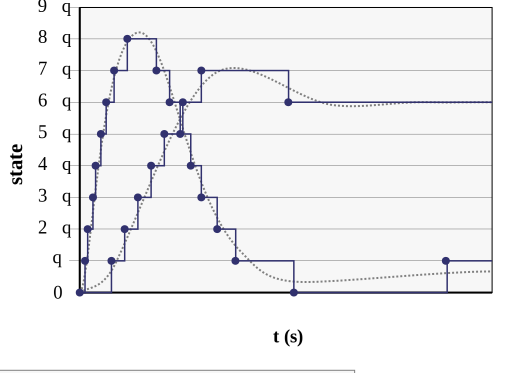
\includegraphics[width=1.0\linewidth]{intro_plots_both.png}
    \caption{Example simulation results for a conceptual $2^{nd}$ order dynamical system, comparing a time-slicing numerical integration method to a quantized state method, where $\Delta t$ is the time step, and $\Delta Q$ is the quantization step size.}
    \label{fig:intro_plots_both}
\end{figure}

In the quantized solution on the right in figure \ref{fig:intro_plots_both}, the quantized state results are not solved synchronously for all system states, and are only defined for each state at multiples of that state's quantization step size ($\Delta Q$). Note that the quantized state solution points are connected with a zero-order hold curve. This is because the results of a $1^{st}$ order quantized state solution are defined as piece-wise constant \cite{kofman2001b} and they are typically rendered accordingly in plots.

\section{Rationale for Applying Quantized State Solutions to Power Systems}

In order to simulate the full range of dynamic behavior in a typical electrical power system with a single dynamical system model, a stiffness ratio ($\lambda_{max} \backslash \lambda_{min}$) of $10^6$ or higher must be supported. Time constants of a power system typically span from the turbo-governor (with time constants on the order of 1 second), to the very fast dynamics of a switching converter (with micro-second time constants). The uniform time-slicing of nodal analysis can potentially simulate such a high-bandwidth system model only by using time steps on the order of micro-seconds. Each of these micro-second time steps requires a full update of the system Jacobian matrix (in the case of non-linear models, which is required for practical, real-world system models). This constant update of the Jacobian matrix forces a constant matrix factorization at each micro-second time step. The computational load (flops per simulation second) for this matrix factorization grows exponentially with increases in system size. For large transmission grids, the electrical node count (and thus the order of the Jacobian matrix) can be as high as hundreds of thousands. Variable time step methods are of little use here, as the simulation of a detailed switching converter requires dense time-slicing between each switch transition, even when the system is in a quasi-steady-state condition.

Quantized state solutions can potentially solve this extreme stiffness problem, and because most of the current literature on quantized state integration revolves around small, linear systems, this is a novel area for research. The simulation of larger, stiffer, and highly non-linear systems is a new area for the application of quantized methods.

\section{Document Outline}

This dissertation will begin in chapter \ref{chap:lim} by describing the Latency Insertion Method, specifically the formulation most relevant to our needs. We cannot apply quantized state solution methods directly to a traditional formulation of a power system. The LIM will allow us to cast the power system model into a form that can be used in a discrete event context by enforcing latency at every system state. The QSS integration concepts are then introduced in chapter \ref{chap:qss}, describing the basic properties of Quantized State Systems. The formal QDEVS specification for a LIM-based system model is then developed in chapter \ref{chap:qdl}, defining the QDEVS functions that operate on a LIM-based system model. The MATLAB and Python implementations of QDL simulations is discussed in chapter \ref{chap:simulator} (with the full source code of these implementations listed in Appendix A).

The next three chapters contain simulations of systems of increasing complexity. Chapter \ref{chap:examples} presents several interesting test cases for the QDL method that demonstrate various properties and advantages of the method. Among these are a 40 state, linear grid of LIM branches and nodes, with an extreme stiffness ratio designed to test the limits of the method. Following those examples, chapters \ref{chap:syncmach} and \ref{chap:powersys} finally apply the QDL method to realistic power system models and systems. Chapter \ref{chap:syncmach} presents a $7^{th}$ order, three-phase synchronous machine attached to an infinite bus. The feasibility of the QDL method for such a model is demonstrated, and the simulation result match the reference simulation very well. The synchronous machine simulation is then used to investigate the relationship between quantization step size and error. Chapter \ref{chap:powersys} applies QDL to a relatively large problem: a multi-machine power system network with 12 device models including cables, buses, a synchronous generator, an induction machine, loads, an (average model) converter, and control devices (an exciter and a governor). This system is complex and realistic enough to test the thesis of this work: to determine if a quantized state method is a feasible and advantageous approach to simulating power system dynamics

Chapter \ref{chap:deltaq} explores the important question of how to select the quantization step size ($\Delta Q$) to optimize simulation performance and control error. A method is proposed to intelligently select $\Delta Q$ based on the propagation of error within the QDL system model. The problems with steady-state behavior of the QDL method is discussed in chapter \ref{chap:steadystate}, along with a proposal for a method of detecting steady-state conditions and mitigating steady-state noise. Finally, chapter \ref{chap:future} describes possible next steps for the research and development of this new method, including further investigation into better methods for selecting $\Delta Q$, a search for better error and noise mitigation, and integrating the most recent, advanced QSS integration methods.
